\documentclass[12pt]{report}
\usepackage[utf8]{inputenc}
\usepackage{xcolor}
\usepackage[margin=1in]{geometry}
\usepackage{soul} 
\usepackage{apacite}
\usepackage{graphicx}
\usepackage{xurl}
\usepackage{subcaption}
\captionsetup{compatibility=false}

\usepackage{fancyhdr}
\pagestyle{fancy}

\lhead{Research Project}
\rhead{Draft Chapter 2}
\cfoot{\thepage}
\renewcommand{\headrulewidth}{0.4pt}
\renewcommand{\footrulewidth}{0.4pt}

\title{Alternate Review Systems:\\ Quantifying Enjoyability in Table-top Games}
\author{Jai Bakshi \\ 21060322069}
\date{November 2024}

\begin{document}
	\maketitle
	\setcounter{chapter}{1}
	\chapter{Effects of Entity Lengths on Game Time}
	This chapter will continue the investigation of the effects of changing various parameters of the classic game of snakes and ladders, aiming to quantify the impact of various game parameters on the overall game dynamics. In this chapter, the research aims to achieve this by simulating numerous games of while systematically varying the lengths of snakes and ladders while keeping the quantities of snakes and ladders on the board as constant values. Much like the previous chapter, in order to make conclusive claims based on the computation and results, the model limits changes in parameters to only affect one category of entities on the board, i.e. the lengths of snakes and ladders. This allows the research to systematically examine how changes in these parameters affect the distribution of game duration - specifically, the number of moves needed to reach the end state.
	
	\section{Setting up the board}
	The game board is modeled as a 100-tile grid, akin to the classic Snakes and Ladders game. The player starts at tile 1, with no requirement to roll a certain number to be let out (i.e., no starting condition), and the goal state is reaching 100 or exceeding it. There are three entities on each board:

	\begin{enumerate}
		\item Agent: The Agent represents the player, the Agent's movement is determined by a fair six-sided dice roll. 
		\item Snake: Each snake has two terminal ends: the head and the tail. When the player lands on the head of the snake, they move down to the tile at the snake's tail.
		\item Ladder: Similar to snakes, ladders have two ends: the base and the top. When the player lands at the base of the ladder, they climb up to the tile at the ladder's top.
	\end{enumerate}

	The nature of these entities is determined by the following controllable parameters:
	\begin{enumerate}
		\item Board Size ($BoardSize$): The maximum size of the board in terms of the number of tiles.
		\item Number of Snakes ($N_{s}$): The total quantity of snakes on the board.
		\item Number of Ladders ($N_{l}$): The total quantity of ladders on the board.
		\item Length of Snakes ($L^{i}_{s}$): This parameter determines the length of the $i^{th}$ snake on the board for $i=1,2,... N_{s}$. It dictates how far down a player moves when landing on a snake's head.
		\item Length of Ladders ($L^{i}_{l}$): This parameter determines the length of $i^{th}$ ladder on the board for $i=1,2,... N_{l}$. It dictates how far up a player climbs when encountering a ladder's base.
		\item Ladder Position ($Ladder^{i}_{base/top}$): The position of the $i^{th}$ ladder's terminal ends.
		\item Snake Position ($Snake^{i}_{head/tail}$): The position of the $i^{th}$ snake's terminal ends.
	\end{enumerate}
	
	To ensure that the board configuration remains valid and doesn't present any conflicts such as - positioning snakes or ladders at invalid tiles where they might go out of the bounds of the board, certain constraints are implemented:
	
	\begin{enumerate}
		\item Ladder Constraint: Ladders cannot begin within the $L^{i}_{l}$ tiles of the board to prevent them from extending beyond the game's end. The ladder's starting position therefore becomes:  $$Ladder^{i}_{start} \leq BoardSize - L_{l}$$
		\item Snake Constraint: Snakes cannot begin within the first $L^{i}_{s}$ tiles to avoid their tails going below the starting position. The snake's end therefore becomes: $$Snake^{i}_{start}\geq 1 + L_{s}$$
		\item Overlap Constraint: To maintain game integrity, no terminal ends of a snake or ladder (start or end) can overlap with any part of another snake or ladder. The paths of snakes and ladders can coincide at various points so long as they don't have overlaps at the ends of the entities. If an overlap occurs, the simulation setup randomly decides whether to remove the overlapping snake or ladder based on a probability of 0.5.
	\end{enumerate}
	
	\section{Approaches to assign $L_s$ and $L_l$}
	For this chapter, three distinct approaches are deployed to assign the lengths of snakes and ladders on the game board. Each approach allows for unique characteristics of the board configuration to facilitate a comparative analysis of game time under varying assumptions. These are as follows:
	\begin{enumerate}
		\item Fixed unequal lengths: This approach involves assigning fixed but unequal lengths to all snakes and ladders, i.e. $L^i_s \neq  L^i_l$ \space $ \forall i \in [1, N]$ and all $L_s$  and $L_l$ are equal to each other.
		\item Sampling from Distributions: This approach makes use of three sampling distributions in order to assign $L^i_s$ \&  $L^i_l$ \space $\forall i \in [1, N]$
		\item Fixed Start and End Points: This diverges from the concept of explicitly calculating and assigning lengths of each snake and ladder, effectively deriving their lengths implicitly.
	\end{enumerate}
	
	\subsection{Selecting unequal $L_s$ and $L_l$}
	This approach provides with a baseline for analyzing gameplay outcomes when the lengths are purely deterministic and ensures uniformity across the experiments. The predefined unequal lengths would act as a control group to assess the impacts other methods of selecting $L_s$ and $L_l$ would have without introducing randomness. it acts as a stable point of reference clear from the effects of other variables and parameters, such as entity placement and dice randomness.
	
	\subsection{Rationale for Length Selection using Sampling Distributions}
	The basis of this chapter of the research project is to study the effects of changing $L_s$ and $L_l$ on the game times while keeping the $N_s$ and $N_l$ constant. Therefore the process of determining lengths of snakes and ladders on the board becomes crucial to understanding the variability in the gameplay and try to look for balance in the same. The selection criteria for the lengths is based on probabilistic sampling methods ensuring that the lengths are diverse while adhering to constraints. The $L_s$ or $L_l$ are sampled using of the three distinct probability distributions:
	\begin{enumerate}
		\item Uniform distribution: All valid lengths between 1 and $L_max$ are equally likely, this ensures an unbiased selection across the entire range of lengths, providing a uniform probability for shorter and longer lengths.
		$$P(L=x)=\frac{1}{L_{max}}, \forall x \in \{1,2,\ldots,L_{max}\}$$
		\item Normal distribution: A Normal/Gaussian distribution is characterized by a mean $\mu$ and a standard deviation $\sigma$, for the lengths of snakes and ladders:
		\begin{itemize}
			\item $\mu$ is set to $\frac{L_{max}}{2}$, placing the most likely lengths near the midpoint of the range
			\item $\sigma$ is set to $\frac{L_{max}}{6}$, which suggests that most lengths fall within the range $[\mu-3\sigma, \mu+3\sigma]$
			$$P(L=x) = \frac{1}{\sqrt{2\pi\sigma^2}}{e^{\frac{(x-\mu)^2}{2\sigma^2}}, \forall x\in[1, L_{max}]}$$
		\end{itemize}
		\item Exponential distribution: This emphasizes on the shorter lengths, with the probability of longer lengths decreasing exponentially. The scaling parameter $\lambda$ is set to $\frac{L_{max}}{3}$ ensuring a reasonable spread of values.
		$$P(L=x)={\lambda}e^{{-\lambda}x}, \forall x \in [1, L_{max}]$$
	\end{enumerate}
	
	For this research, the $L_{max}$ has been set to 40. This is done to ensure that there aren't any outlier snakes or ladders which remain extremely long (spanning from the top to the bottom of the board). Also, to ensure that the generated lengths are valid and abide the by game rules, the aforementioned constraints are applied.
	
	\subsection{Assigning Fixed Start and End points}
	This approach diverges from directly controlling the $L_s$ and $L_l$. Instead, it involves assigning randomized $Ladders^i_{start/end}$ and $Snakes^i_{start/end}$. This approach to the problem introduces another layer of variability by purely focusing on their placement rather than predetermined or sampled lengths.
	For each snake, the $Snake^i_{start}$ is chosen from the range $[2, BoardSize - 1]$ abiding by the snake constraint. While, the $Snake^i_{end}$ is determined by randomly selecting tile below its starting position, i.e. $$1\leq Snake^i_{end} < Snake^i_{start}$$ 
	For ladders, the $Ladder^i_{start}$ is chosen randomly from $[2, BoardSize - 1]$ keeping the ladder constraint in check, whilst its $Ladder^i_{end}$ is assigned randomly above its starting position, i.e. $$Ladder^i_{end}>Ladder^i_{start}$$ 
	
	By decoupling length from predetermined distributions, the method accommodates a wider variety of configurations, making it suitable for exploring edge cases in gameplay. The method allows for a high degree of randomness in gameplay and will be used to test the robustness of the study, offering insights into how random placement and implicit lengths impact game duration, difficulty, and variability.
	
	\section{Presenting Findings}
	The simulations represent the probabilistic nature of snakes and ladders, with the outcome largely being determined by the interplay between board design, entities and inherent randomness in the dice rolls. The board design consists of a number of Snakes and Ladders with varying lengths that either move the player down or bring them closer to the goal.  This section of the chapter focuses on how the $L_{s}$ and $L_{l}$ affects the average game time. Across the three major approaches, and by using the simulated data, this chapter explores the relationship between different configurations of snakes and ladders, keeping $N_l$ and $N_s$ constant (10 each) while varying their lengths. The game has been simulated 1000 times with 10 distinct board configurations while varying the parameters independently of each other.
	\subsection{Controlled Approach: Unequal $L_{s}$ and $L_{l}$}
	\begin{figure}
		\centering
		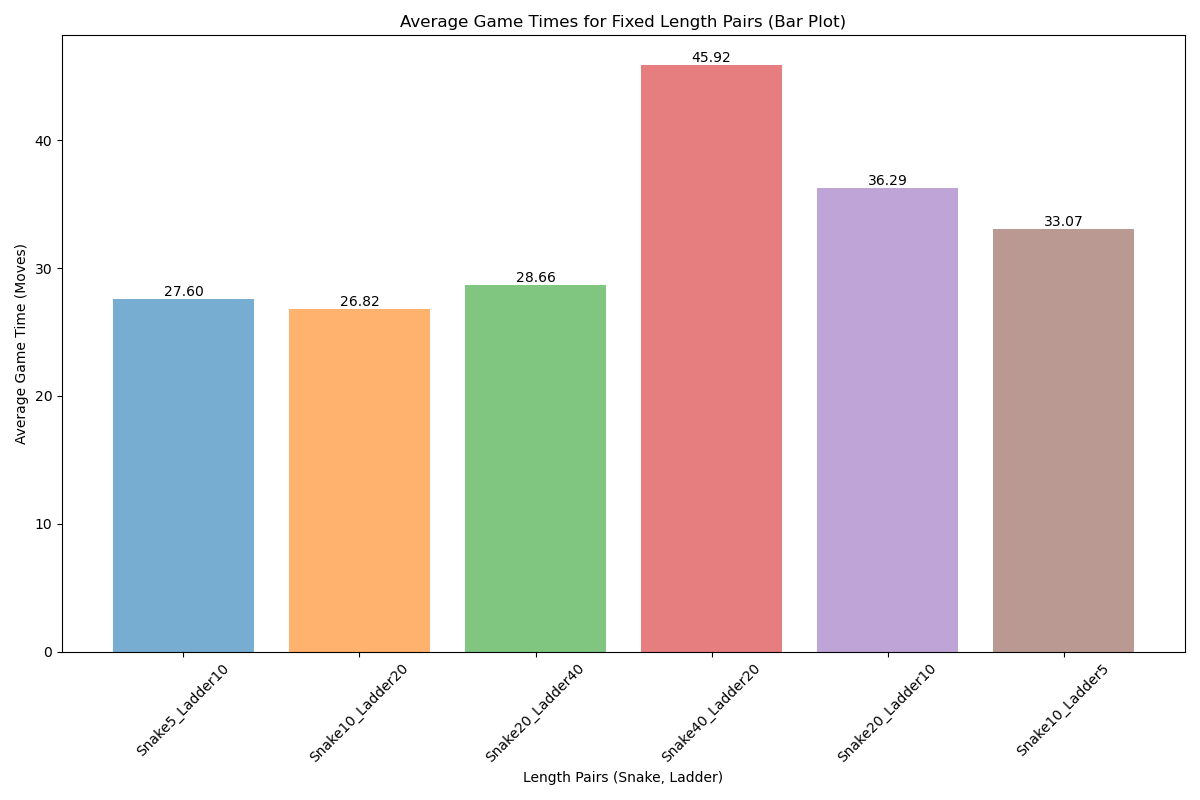
\includegraphics[width=0.5\textwidth]{../withLength/UnequalLengths/approach_1_fixed_length_pairs_barplot}
		\caption{Average Game Times for Fixed Unequal Lengths}
		\label{fig:approach1fixedlengthpairsbarplot}
	\end{figure}	
	\begin{figure}[h]
	\centering
	\begin{subfigure}[b]{0.32\textwidth} 
		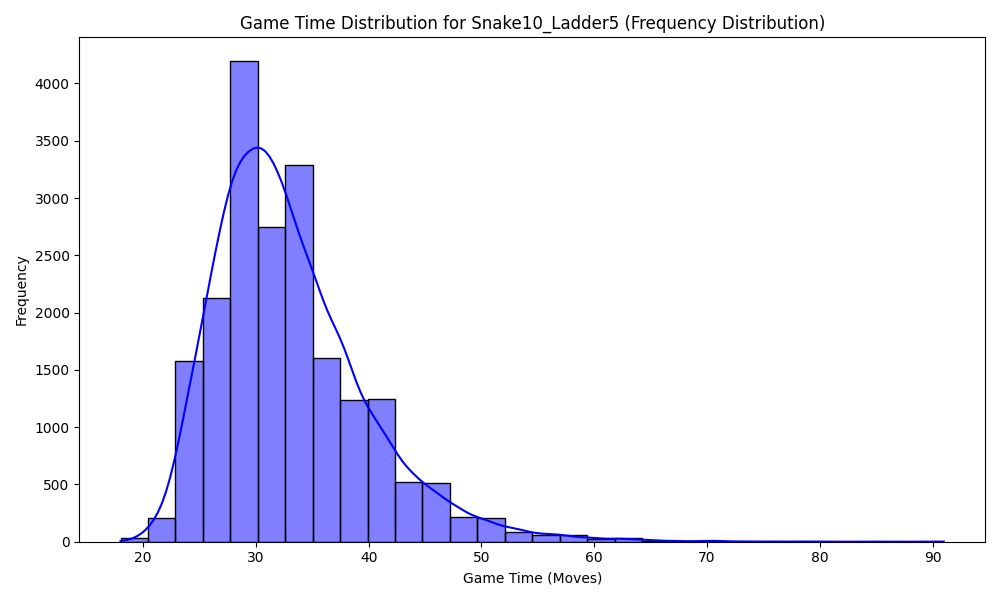
\includegraphics[width=\linewidth]{../withLength/UnequalLengths/game_time_distribution_Snake10_Ladder5}
		\caption{$L_s = 10$, $L_l = 5$}
	\end{subfigure}
	\hfill
	\begin{subfigure}[b]{0.32\textwidth}  
		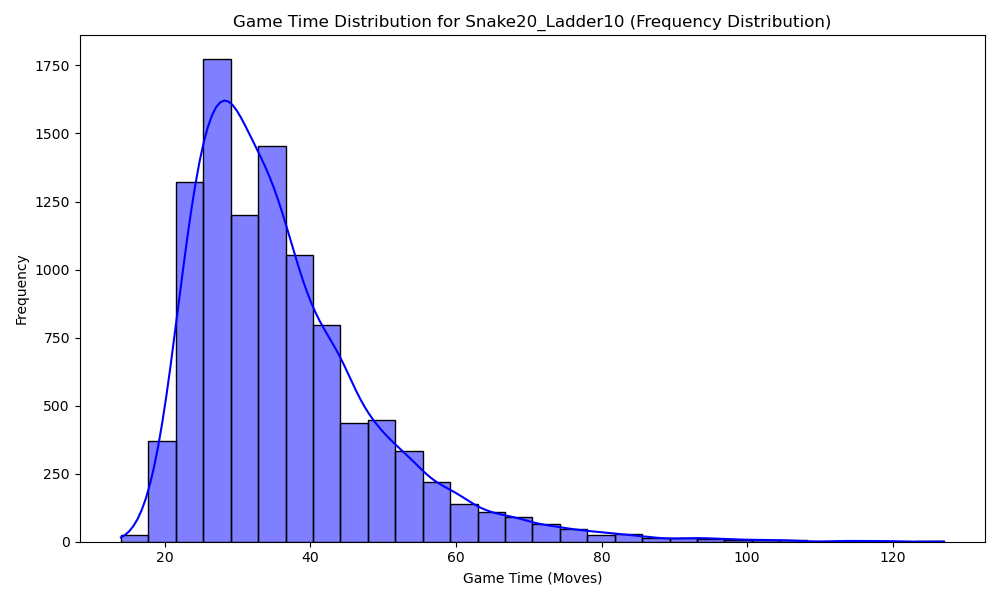
\includegraphics[width=\linewidth]{../withLength/UnequalLengths/game_time_distribution_Snake20_Ladder10}
		\caption{$L_s = 20$, $L_l = 10$}
	\end{subfigure}
	\hfill
	\begin{subfigure}[b]{0.32\textwidth}  
		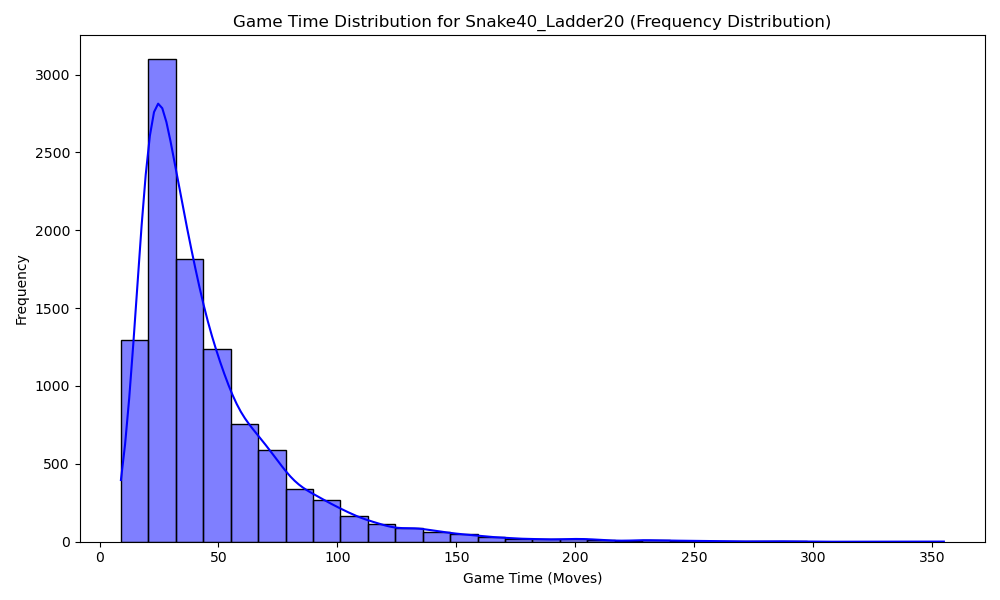
\includegraphics[width=\linewidth]{../withLength/UnequalLengths/game_time_distribution_Snake40_Ladder20}
		\caption{$L_s = 40$, $L_l = 20$}
	\end{subfigure}
	\caption{Game Time Distributions for Configurations with $L_s > L_l$}
	\end{figure}
	This section makes use of fixed the unequal $L_{s}$ and $L_{l}$ across 10 different board configurations each and 1000 simulations ran for each board layout. In this controlled approach, we systematically varied the $L_{s}$ and $L_{l}$. The lengths were assigned in pairs, ensuring that the $L_{s}$ and $L_{l}$ were not equal. This approach allows the analysis to isolate the impacts of length variation on game time. The bar plot (Figure 2.1) illustrates the average game times for various pairs of lengths. It is observable that the average game time generally increased as $L_s - L_l$ increases positively. This suggests that when snakes are significantly longer than the ladders, players will tend to experience more setbacks in their positions, therefore contributing to longer game times on average. There is no real observable impacts to the game times across pairs that have $L_l > L_s$. The frequency distribution plot (Figure 2.2 (c)) provides a detailed overview of the game time distribution for all the simulations conducted in the specific configuration ($L_s=40$ \& $L_l=20$). The distribution appears to be heavily right-skewed, indicating that most games end within a moderate number of moves, whilst there are occasional occurrences of significantly longer games. This skew is most likely due to the nature of dice rolls and how often the agent comes into contact with snakes despite there being ladders that are long enough. When configurations with $L_l > L_s$ are compared against one another, it can be observed that the configurations where $L_l - L_s < 20$ their spread is much tighter and looks like the normal distribution with few outliers. The average game time across these simulations also seems much closer to one another unlike the huge spikes observed in Figure 2.1.

	\begin{figure}[h]
		\centering
		\begin{subfigure}[b]{0.32\textwidth} 
			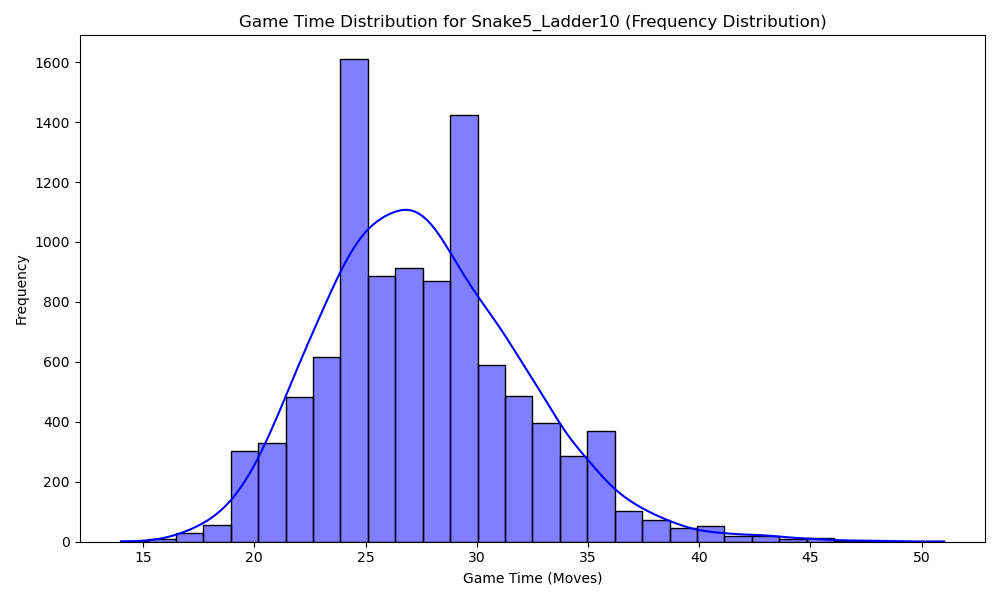
\includegraphics[width=\linewidth]{../withLength/UnequalLengths/game_time_distribution_Snake5_Ladder10}
			\caption{$L_s = 5$, $L_l = 10$}
		\end{subfigure}
		\hfill
		\begin{subfigure}[b]{0.32\textwidth}  
			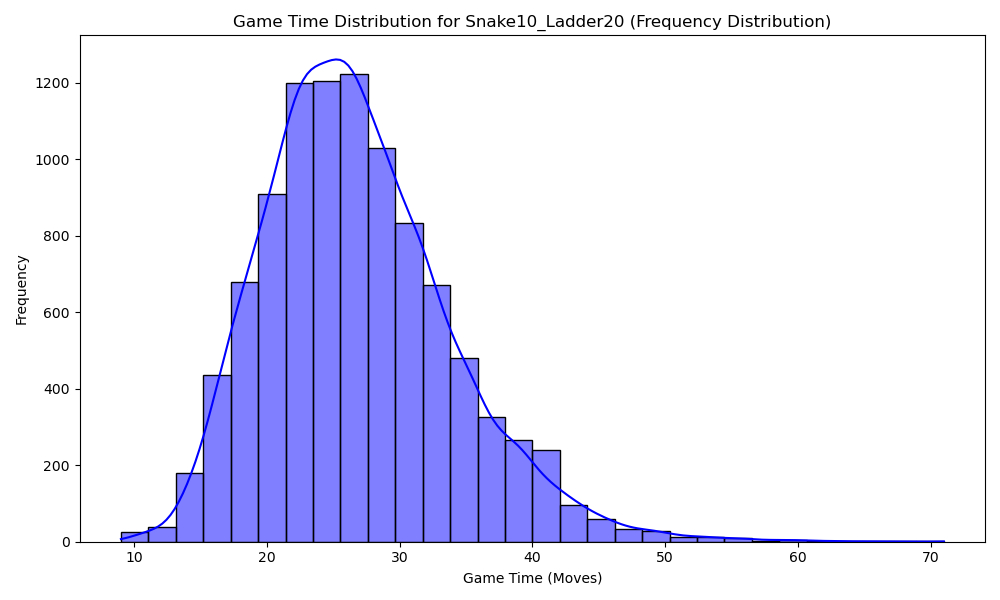
\includegraphics[width=\linewidth]{../withLength/UnequalLengths/game_time_distribution_Snake10_Ladder20}
			\caption{$L_s = 10$, $L_l = 20$}
		\end{subfigure}
		\hfill
		\begin{subfigure}[b]{0.32\textwidth}  
			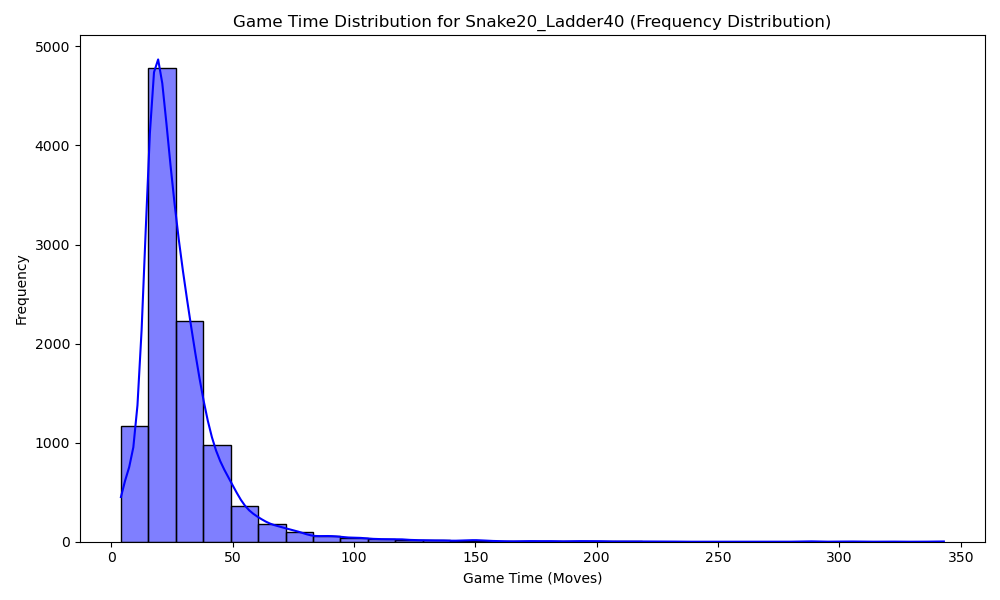
\includegraphics[width=\linewidth]{../withLength/UnequalLengths/game_time_distribution_Snake20_Ladder40}
			\caption{$L_s = 20$, $L_l = 40$}
		\end{subfigure}
		\caption{Game Time Distributions for Configurations with $L_l>L_s$}
	\end{figure}
	
	\subsection{Using Sampling Distributions}
	This section delves into the effects of different sampling distributions on  $L_{s}$ and $L_{l}$. It explores three statistical distributions: uniform, normal, and exponential, each with $N_s, N_l=10$, where the  $L_{s}$ and $L_{l}$ were sampled from their respective distributions. For each distribution, 1000 games were simulated on 10 different boards. Figure 2.4 shows the aggregated averages of game times across the three sampling distributions. Here, the highest average game time stems from the exponential sampling method, followed by normal distribution and the uniform distribution fetching the lowest average game time. Sampling from the exponential distribution nets out more lengths that are smaller, whilst there still remains a lower chance of having longer entities on the board, this suggests that having more $N_s$ \& $N_l$ with smaller lengths cause the games to go on for longer. Meanwhile, the normal distribution allows for the $L_{s}$ and $L_{l}$ to be sized around between $[\mu \pm 3\sigma]$, where $\mu$ \& $\sigma$ are determined by the $L_{max}$. The simulations run under normal sampling present to be a much more stable set of configurations with lower game times. Due to the more randomly assigned lengths under the uniform sampling method, it shows a longer game on average.
	\begin{figure}
		\centering
		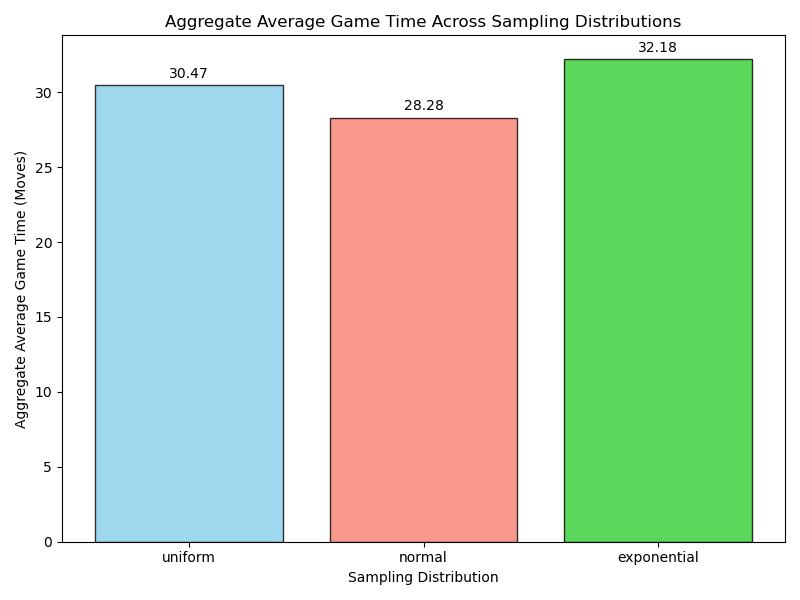
\includegraphics[width=0.6\linewidth]{../withLength/FinalSampling/comparative_aggregate_average_game_times}
		\caption{Aggregated Averages of Game Time across the sampling distributions}
		\label{fig:comparativeaggregateaveragegametimes}
	\end{figure}
	Figure 2.5 displays the frequency distributions of game times for a fixed layout under each sampling method. It's observable that all the three distributions exhibit right-skewness indicating while most games finish in a moderate set of moves, there may be outliers in some runs. The highest variability also can be seen in the set of simulations run under the exponential sampling, this can be attributed to the nature of smaller entities on the board, but also their placement. Figure 2.6 (b) suggests that across most boards that were generated using exponential sampling the average number of moves taken to end the game was consistently higher than any of the other boards. Figure 2.6 (a) shows that while the average number of moves remained more or less similar across most board layouts, there were a few boards with quite high averages. And, lastly the normal distribution shows the most variability across the boards played but the average game time was consistently low and very few outliers could be seen that pushed the game time upwards.
	\begin{figure}[h]
		\centering
		\begin{subfigure}[b]{0.32\textwidth}
			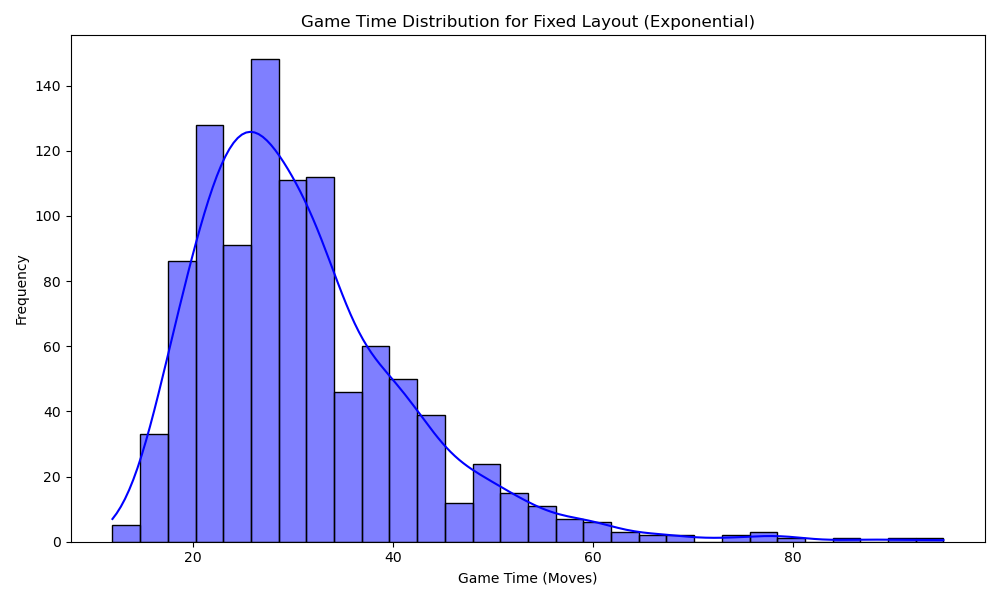
\includegraphics[width=\linewidth]{../withLength/FinalSampling/full_distribution_exponential}
			\caption{Exponential Distribution}
		\end{subfigure}
		\hfill
		\begin{subfigure}[b]{0.32\textwidth}
			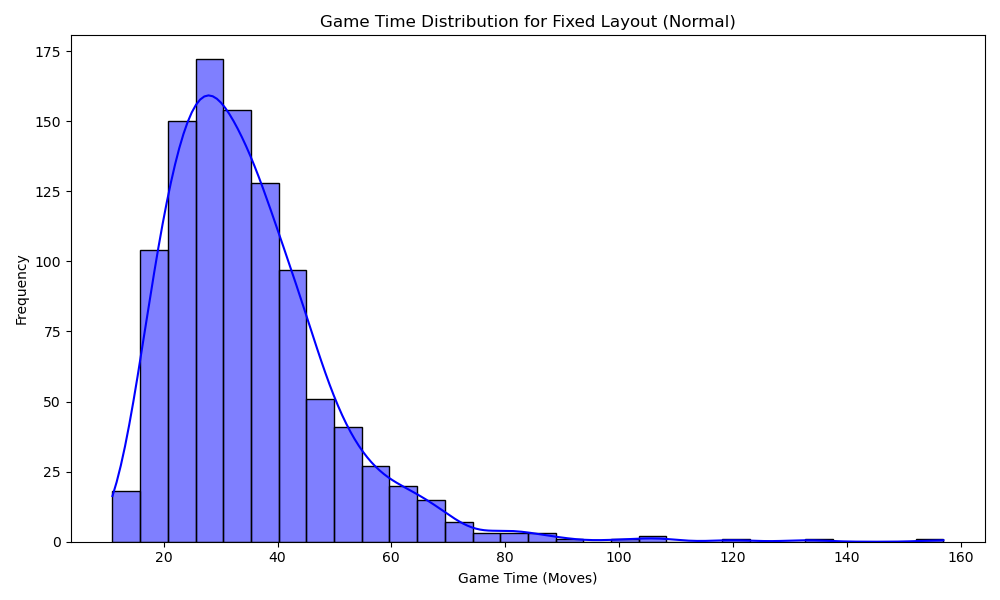
\includegraphics[width=\linewidth]{../withLength/FinalSampling/full_distribution_normal}
			\caption{Normal Distribution}
		\end{subfigure}
		\hfill
		\begin{subfigure}[b]{0.32\textwidth}
			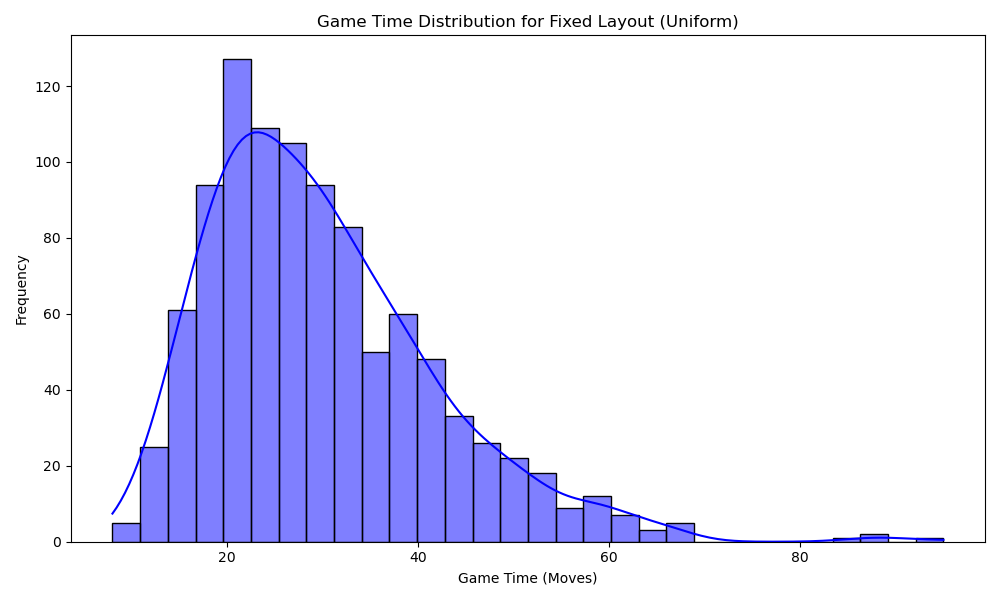
\includegraphics[width=\linewidth]{../withLength/FinalSampling/full_distribution_uniform}
			\caption{Uniform Distribution}
		\end{subfigure}
		\caption{Game Time Distributions for a Fixed Layout, by Sampling Method}
	\end{figure}

	\begin{figure}[h]
		\centering
		\begin{subfigure}[b]{0.32\textwidth}
			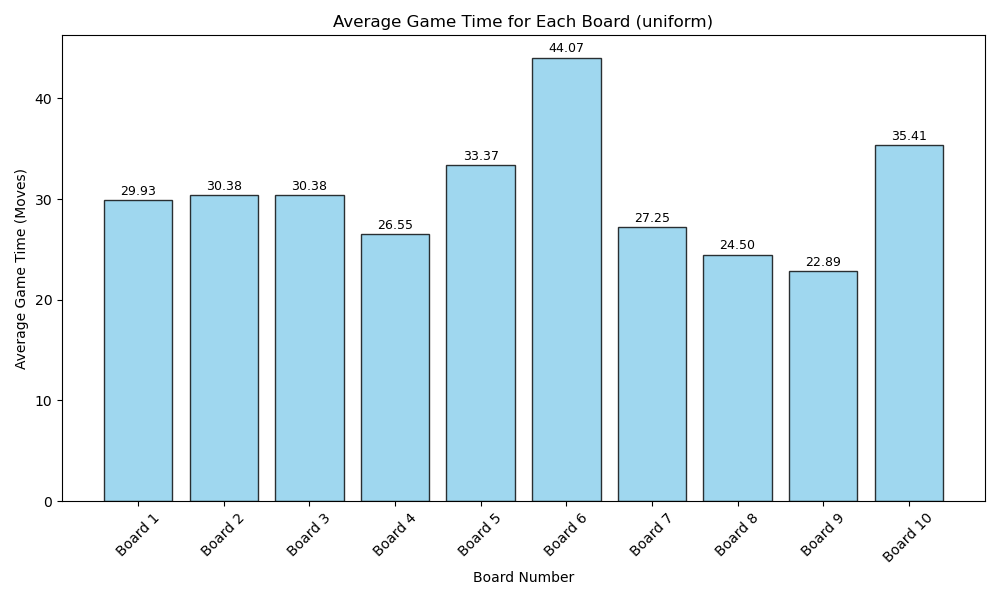
\includegraphics[width=\linewidth]{../withLength/FinalSampling/board_averages_uniform}
			\caption{Uniform Distribution}
		\end{subfigure}
		\hfill
		\begin{subfigure}[b]{0.32\textwidth}
			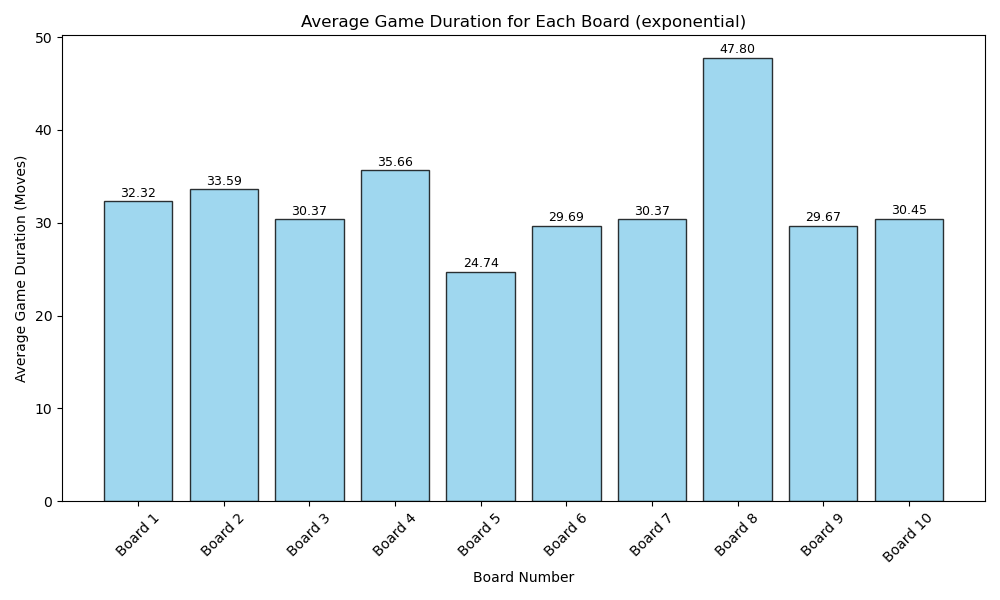
\includegraphics[width=\linewidth]{../withLength/FinalSampling/board_averages_exponential}
			\caption{Exponential Distribution}
		\end{subfigure}
		\hfill
		\begin{subfigure}[b]{0.32\textwidth}
			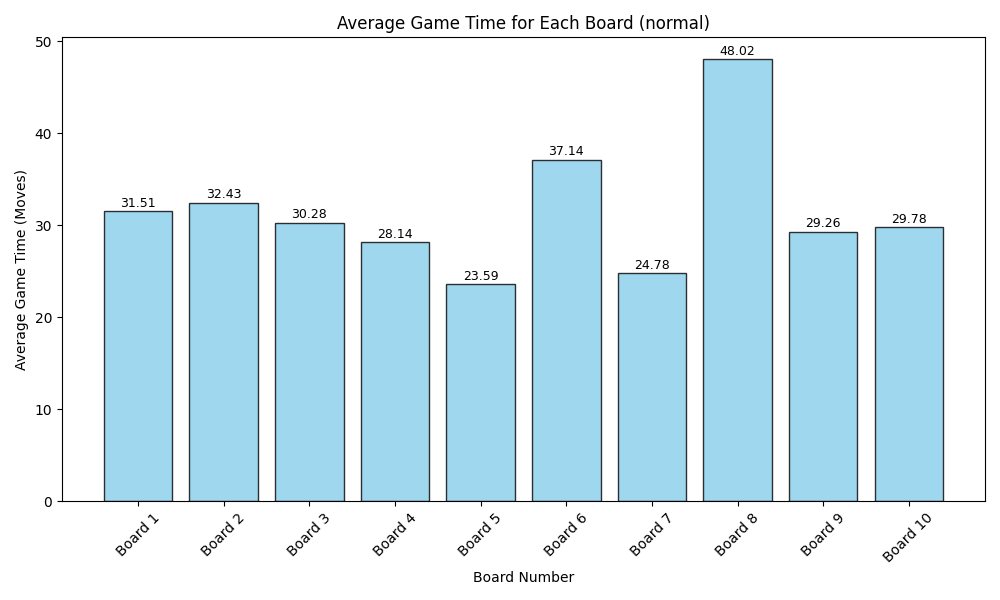
\includegraphics[width=\linewidth]{../withLength/FinalSampling/board_averages_normal}
			\caption{Normal Distribution}
		\end{subfigure}
		\caption{Average Game Time for Each Board, by Sampling Distribution}
	\end{figure}
	Therefore, the exponential distribution, with its propensity for generating longer lengths, generally leads to higher average game times and greater variability. The normal distribution provides a more balanced approach, while the uniform distribution results in the shortest average game times and the most predictable length distribution. 
	
	\subsection{Randomly Generated Boards}
	This subsection looks at the effect of randomly generated snakes and ladders based on $Ladder_{start/end}$ \& $Snake_{start/end}$ positions. These positions are generated while keeping the length constraints into consideration. This approach adds more variability as compared to previous approaches where the lengths were first controlled. Figure 2.7 (a) illustrates the average game times across 10 different boards generated while following the random assignment for this approach. Each bar represents the average game time for each specific board and it can be seen that variability in average game times across the boards is quite evident. The average across boards range from nearly 22 to 40 moves. Figure 2.7 (b) shows the frequency distribution of game times across all the games, and it is indicative of the same variability as well, as evident by the random spikes in certain sections and the kernel density line as well. Certain boards, due to the specific configuration of snakes and ladders, may present more challenges or opportunities for the agent, leading to longer or shorter games, respectively. This could be due to the nature of the computation as well. While lengths were randomly assigned across a smaller range of values in the previous approach, this approach allows the simulations to pick and choose random start and end positions which have far more range to be chosen from. It could be possible that on some boards, most of the snakes and ladders were more densely populated close to one another, whilst some may have them widely spread apart. This would affect the agent's movement significantly, since, boards with more widely spread apart entities, have a higher chance for them to be triggered, whilst more densely populated boards have a tendency where most entities might get skipped due to the lengths of the entities. 
	\begin{figure}[h]
		\centering
		\begin{subfigure}[b]{0.48\textwidth}
			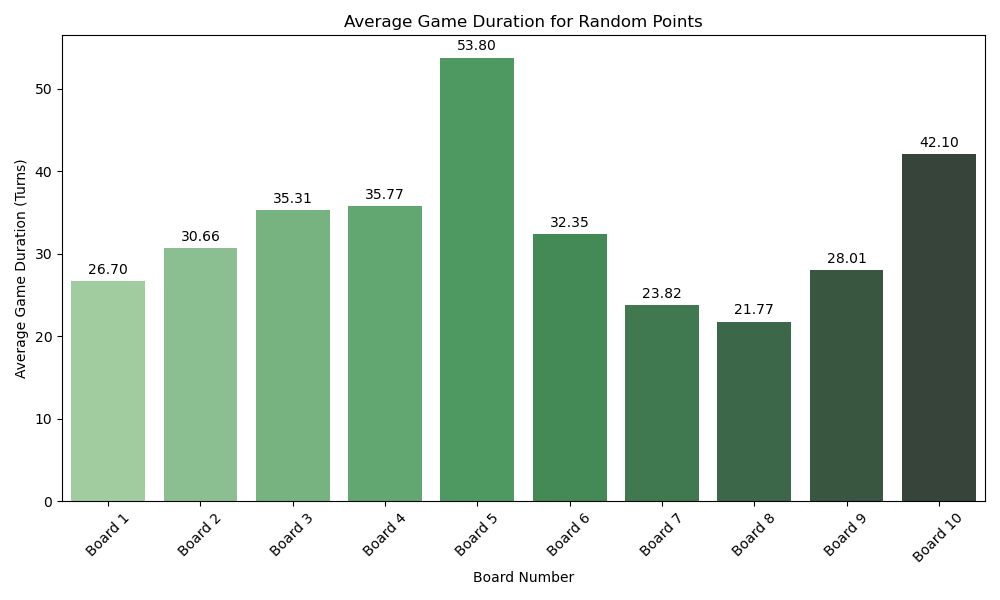
\includegraphics[width=\linewidth]{../withLength/RandomLength/approach_3_random_points}
			\caption{Average Game Time for Random Points}
			\label{fig:approach3randompoints}
		\end{subfigure}
		\hfill
		\begin{subfigure}[b]{0.48\textwidth}
			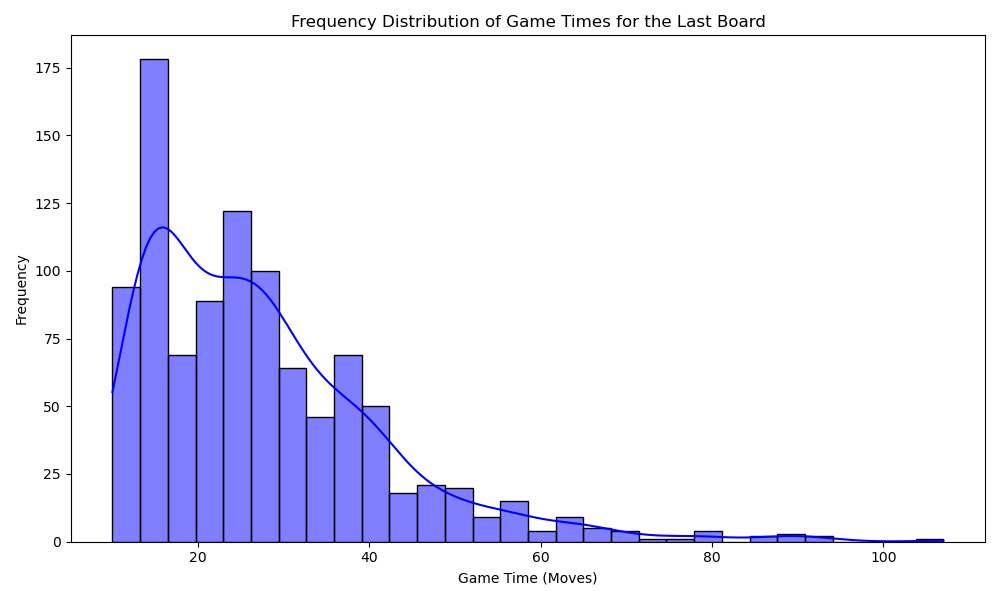
\includegraphics[width=\linewidth]{../withLength/RandomLength/approach_3_game_time_distribution}
			\caption{Frequency Distribution of Game Times}
			\label{fig:approach3gametimedistribution}
		\end{subfigure}
		\caption{Analysis of Randomly Generated Boards}
	\end{figure}
	
		\section{Further Attempts at Modeling}
	To investigate the dynamics of the game even further, the research seeks to employ a Markov model in the coming chapters. Markov models are most suited to analyse stochastic processes where the future states depend on the current state of the agent, making them a great fit for the game of Snakes and Ladders. In the suggested model, each tile would represent a state in the Markov chain. Transitions between states will be determined by the probabilities of dice rolls and the positioning and effects of the entities on the board, namely, the Snake and the Ladder. By constructing an appropriate transition matrix and analyzing its properties, it would be possible to gain insights into various aspects of the game mechanics, calculate an expected game duration for any board configuration, understand the dynamics of probabilities of landing on specific tiles of a the board from any point on the board, identify zones or specific tiles that would rarely be traversed and judge the overall effects on the entities on the board. The Markov model should be able to compliment the simulation-based approach that has been conducted thus far, offering a more analytical framework to understand the dynamics of the game.
	
	\section{Analysis and Conclusion}
	This chapter has taken a look at the impacts of $L_s$ and $L_l$ on the game dynamics by trying to run the simulations with three different approaches, either by statically assigning them lengths, or by statistically sampling $L_s$ and $L_l$ based on exponential, normal and uniform distributions and lastly, by completely randomizing start and end points. The findings have seemingly revealed that the lengths have a significant effect on the average game times, and the variability in game time across various configurations. Here, longer snakes tend to prolong games, whilst longer ladders can aid the progress of the agent across the board, thereby increasing or reducing the game time significantly. It was also noticed that the choice of sampling distributions to decide the lengths also play a major role in the game dynamics. Exponential distributions lead to high variability in game times and  make the player sit through significantly longer games, whilst other distributions provide a more balanced and stable approach to assigning these entities their lengths.
	These insights have great implications on game design and balancing, which could in turn allow game designers to fine-tune how challenging games can be and adjust what they would like the game duration to be, especially for games that present a similar model to Snakes and Ladders which have simpler and fewer mechanics. It also showcases how by isolating parameter adjustments categorically can help pinpoint mechanics that may be posing an issue to game enjoyment in terms of game dynamics and the player experience. This chapter also seeks to lay groundwork for future research that would be making use of Markov models to provide a more nuanced understanding of the game. 
	
	\end{document}
	